\documentclass[12pt]{article}
\usepackage{amsmath, graphicx, float, tabularx, booktabs}
\usepackage[table]{xcolor}
\usepackage[margin=1in]{geometry}

\graphicspath{ {images/} }
\rowcolors{2}{gray!25}{white}

\begin{document}

\title{TCP/IP Data Transmission}
\author{Devin Trejo \tabularnewline devin.trejo@temple.edu }
\date{}
\maketitle

\section{Summary}
Today we introduce the TCP/IP, a standard communication network protocol 
commonly used when communicating over the internet and other computer 
networks. The TCP/IP protocol guarantees the message being sent by a server 
is received by a client without error. We will look at a simple application
of the protocol using a PIC32 Microcontroller Unit (MCU) as a server and 
a Windows machine as a client. By analyzing the raw Ethernet frame 
transmission of the TCP/IP messages we better the understanding of how 
TCP/IP successfully transmits data. The analysis of the frames show how 
a client first establishes a socket connection to a server, then sends a 
command to the server, and finally completes the communication medium by 
waiting for a response back from the server. The TCP/IP protocol has some 
overhead messages on top of the messages sent by the client to ensure data 
integrity on both sides.  

\section{Introduction}
The TCP/IP stack is an internet protocol that sets a standard for computers
to communicate over an inter-connected network. Starting a communication 
channel requires a server and a client. The server is setup to listen for 
connection requests from clients. When a connection attempt is seen the 
server accepts and establishes a connection to the client. The client can 
then request information from the server over the established connection.

The information is sent using the established TCP/IP protocol. TCP/IP is a 
five layered modular protocol. Each part is independent from the other 
allowing for the different pieces to be updated to newer standards without 
having to update the entire protocol. The highest abstraction of the TCP/IP 
protocol is the application layer. In the application layer we see how a 
typical user interacts with the communication protocol. You may be familiar 
with HTTP, SSH, or FTP which are all application layer protocols. 

The application layer hands off communication to the transport layer which 
appends a TCP header to the transmission. The TCP header contains 
information such as a data checksum, destination port, and priority 
pointer to the transmission. In short the TCP header ensure the 
transmission between the server and client arrives in prompt and correct 
fashion. With the TCP header attached to our data our data unit is now 
named a segment.

\begin{figure}[H]
    \centering
    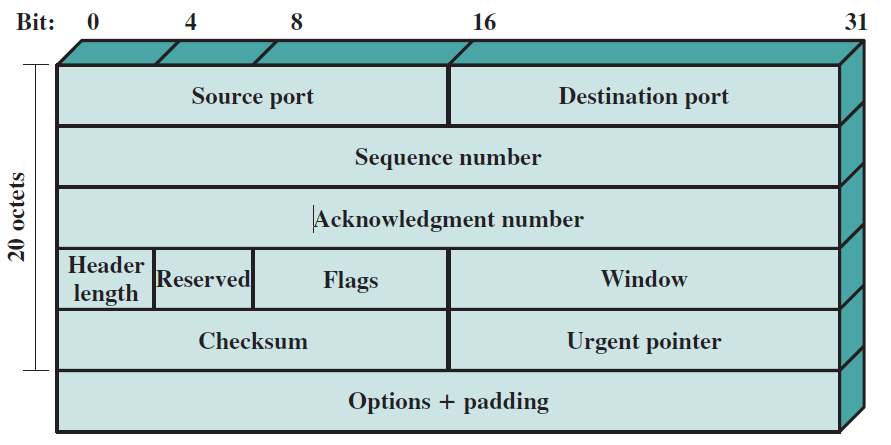
\includegraphics[width=4.5in]{tcp_header.png}
    \caption{TCP Header \cite{Stallings}}
\end{figure}

Next down in the TCP/IP protocol stack is the internet layer. Inside the 
internet layer we append a routing header which tells the packet where to 
go using an IP address (a logical address). An IP address can be either 32 
bits (IPv4) or 128 bits (IPv6) in length. The IP standard also allocates 
space in the header for time to live information. 

\begin{figure}[H]
    \centering
    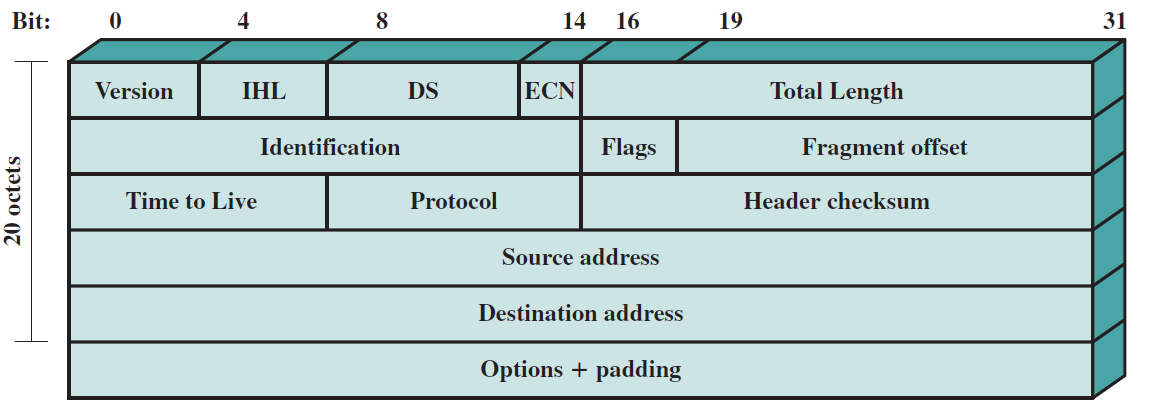
\includegraphics[width=4.5in]{ipv4_header.png}
    \caption{IPv4 Header \cite{Stallings}}
\end{figure}
\begin{figure}[H]
    \centering
    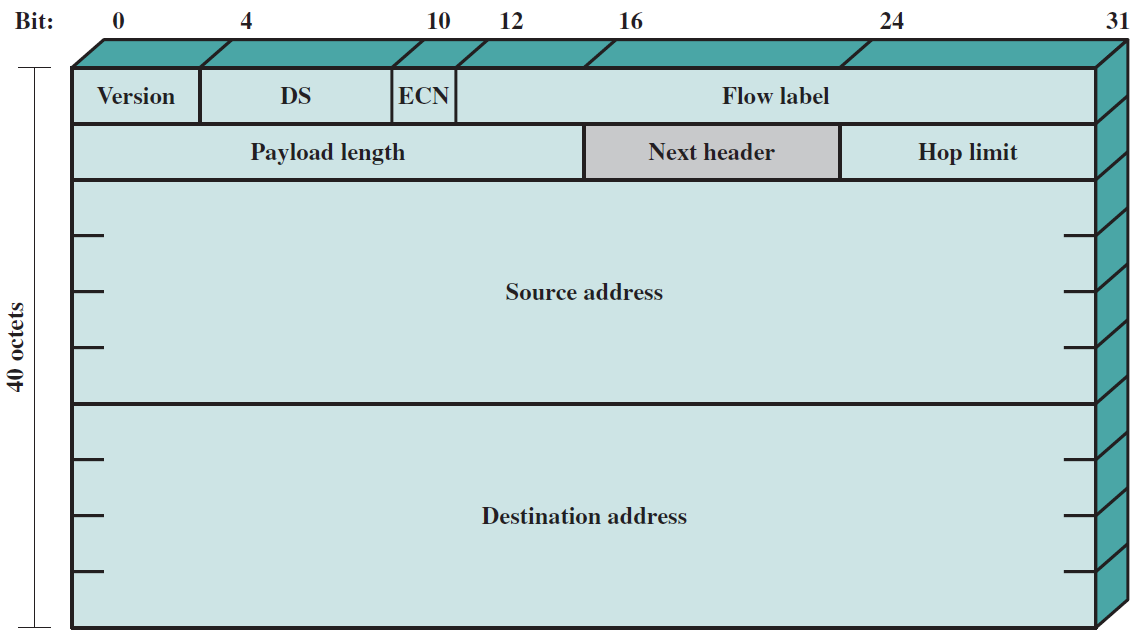
\includegraphics[width=4.5in]{ipv6_header.png}
    \caption{IPv6 Header \cite{Stallings}}
\end{figure}

At this point our information is called an IP packet. An IP packet 
transforms to a frame with the inclusion of a network access/data link 
header. This header contains maps the logical address to a physical address 
within in the network. The different data link standards you may be 
familiar with include Ethernet, Wi-Fi or ATM.

At this level in the stack we reach the bottom most layer called the 
physical layer. The physical layer is consist of the twister pair, fiber 
or microwave communication methods commonly used to transmit data between 
two locations. 

In this project we will investigate the process of using the TCP/IP 
protocol for data communication between a Windows 10 desktop and a 
Microchip PIC32 microcontroller unit (MCU). Our PIC32 will serve as our 
server machine and the desktop will be our client. We will interact with 
TCP/IP using a precompile Visual Basic (VB) application. Our server will 
use a preloaded C program to provide information requested from our VB 
application - there is no server side application. We will use Wireshark, 
a network protocol analyzer program, to identify packets as they cross
through our network to see the raw TCP/IP frames. We will identify the 
blocks that make up our transmission.

\section{Discussion}
We begin by programing our PIC32 MCU with server code that is built to 
interact with our VB application. To begin we need to setup our sockets to 
use the TCP/IP protocol and luckily in C there are predefined variables 
that allow us to specify how we will use a TCP, and IPv4 header. Since we 
are using IPv4 we need to define the server’s IP address. Line 34 defines 
the server’s static IP of $192.168.2.105$. Addressing the TCP header is 
seen in line 73 when we tell our socket to use the $SOCK\_STREAM$ 
pre-defined header. $SOCK\_STREAM$ is a predefined data type that 
initializes our TCP header.  Shortly following our $SOCK\_STREAM$ definition
we specify the socket to monitor port ‘6643’ for connections attempts 
being made by our client machine. Defining these constants we now have 
set our server to listen for incoming connections and accept any attempts 
made a by client. After the handshake between server and client is 
established we use the $recvfrom$ C function to receive information 
requests from the client. 

Moving over to our client machine we go to the network configuration set it 
to have a static IP of $192.168.2.102$. We are using the precompiled VB 
program as our application level interaction between the server and client. 
We know from setting up the server that our server IP is $192.168.2.105$ 
and sever listening port is $6653$. By pressing the $Connect$ button we 
create a socket and connect to our server on the client side. 

\begin{figure}[H]
    \centering
    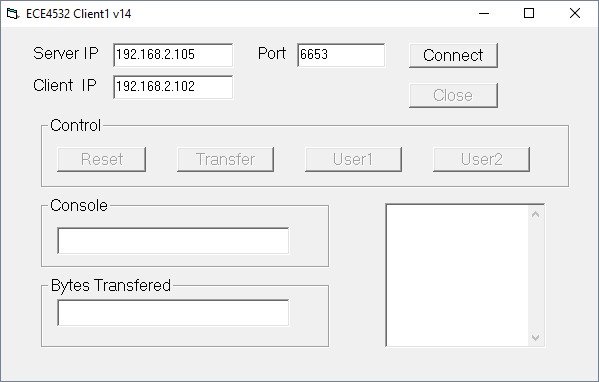
\includegraphics[width=4.5in]{vb_client_intial_setup.png}
    \caption{Client Side VB Program Initial Setup}
\end{figure}

Upon connection attempt we see all three LEDs on our PIC32 board 
sequentially flash. This behavior was defined in our C program which we 
loaded onto the PIC32 board earlier. Moving to the Wireshark program we 
can see the two packets over our network showing the interaction between 
client and server. 

\begin{figure}[H]
    \centering
    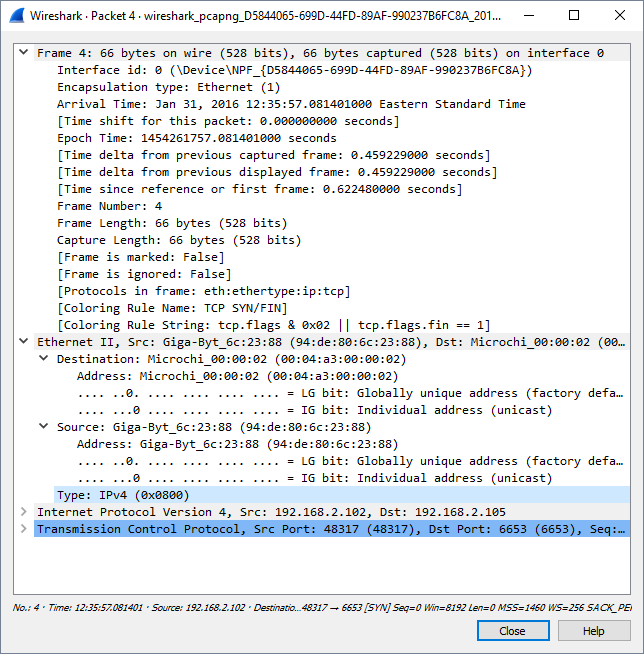
\includegraphics[width=4.5in]{client_server_frame_analysis.png}
    \caption{Client $\rightarrow$ Sever Frame Analysis}
\end{figure}

By clicking connect on our sever we initiated a TCP packet to our server. 
We can see first and foremost that 66 bytes were sent in this frame over 
the Ethernet protocol. At the data-link layer we can see the physical MAC 
addressing of the destination MicroChip PIC32 MCU $00:04:a3:00:00:02$ 
server and source Gigabyte Manufactured client machine $94:de:80:6c:23:88$. 

Moving up to the internet layer we can see the logical IPv4 mapping to the 
server destination $192.168.2.105$ from our client machine $192.168.2.102$. 
Moving up to the transport layer we see the segment is using the TCP 
protocol to send the data. The request on the client sever originated from 
port $48317$ and was sent to the PIC32 sever port $6653$ as specified in
our VBapplication. 

Moving back to our VB application we have two more control buttons; ‘Reset’ 
and ‘Transfer’. To understand the operation of these two buttons we move 
back to our sever source code. Inside our sever-side code we are interested 
in looking at line 115. Here we use the $recvfrom$ function to store our 
received data seen on our predefined socket $StreamSock$ into the buffer 
$rbfr$. We set the output of $recvfrom$ to $rlen$ which we will use to check 
the size of received data. If $rlen$ equals zero it means the client closed 
the socket connection. If $rlen$ is less than zero it means there was an 
error in the connection and the connection to the client was lost. If 
$rlen$ is greater than zero it means the client sent some data which we 
will wish to read. 

To check what was sent by the client we have look at the first byte in the 
transmission. If the received message starts with $2$ we know the sent data 
is the start of a transmission. If the second byte is $71$ we say the 
message sent by the client was a global reset. The global reset status 
sent by the client prompts the sever PIC32 board to blink LED1. We can test 
the function by hitting reset in the VB application and monitoring the 
output on Wireshark. We can see the reset call sent out by the VB 
application by looking at the raw HEX values inside the packet. The first 
54 octets of the packet are reserved for headers that make up our resulting 
transmission frame. The last 3 octets in the frame make up the data of our 
transmission. Note how the transmission begins with the expected 02. We 
then see a $0x47$ which translates to a 71 in decimal. The message in this 
frame is to tell the server to reset the connection. 

\begin{figure}[H]
    \centering
    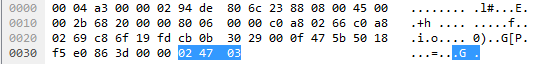
\includegraphics[width=4.5in]{wireshark_raw_hex_frame_sent_reset.png}
    \caption{Wireshark RAW HEX of Frame Sent on Reset}
\end{figure}

The server responds to the client by sending an ACK or Acknowledgment 
packet back. The ACK packet tells the client machine that the server 
successfully received the message. If an ACK was not seen the client would 
start retransmission of the reset packet. 

\begin{figure}[H]
    \centering
    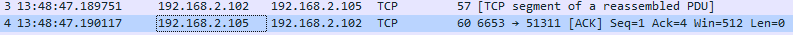
\includegraphics[width=4.5in]{wireshark_packet_listing_of_ACK.png}
    \caption{Wireshark Packet Listing of ACK packet.}
\end{figure}

If the second byte in the received buffer $rbfr$ is equal to $84$ we say 
the client sent a transfer request. The transfer request prompts the PIC32 
board to start generating 1296~bytes worth and load it into our transport 
buffer $tbfr$. The actual loop will generate an array of numbers from zero 
to one thousand two hundred ninety-six. It is shown in both decimal and 
hex in table~\ref{table:txdata}.

\begin{table}[H]
    \centering
    \begin{tabularx}{\textwidth}{|*{3}{>{\centering}X|}}
        %\rowcolor{gray!50}
        %\textit{\textbf{tbfr}} &
        %\textit{\textbf{Decimal}} &
        %\textit{\textbf{HEX}} \tabularnewline
        \toprule
        \multicolumn{1}{|c|}{\textit{\textbf{tbfr}}} & 
        \multicolumn{1}{|c|}{\textit{\textbf{Decimal}}} &
        \multicolumn{1}{|c|}{\textit{\textbf{HEX}}} \tabularnewline
        \midrule
        \textbf{tbfr [0:1]}         & 01    & 0x0001 \tabularnewline
        \textbf{tbfr [2:3]}         & 03    & 0x0003 \tabularnewline
        \textbf{tbfr [254:255]}     & 255   & 0x00FF \tabularnewline
        \textbf{tbfr [256:257]}     & 0257  & 0x0001 \tabularnewline
        \textbf{tbfr [1293:1294]}   & 01293 & 0x000D \tabularnewline
        \textbf{tbfr [1295:1296]}   & 01295 & 0x000F \tabularnewline
        \bottomrule
    \end{tabularx}
    \caption{tbfr Tx Data Generated by PIC32}
    \label{table:txdata}   
\end{table}

\begin{thebibliography}{9}

\bibitem{Stallings} JW. Stallings, Data and Computer Communications, 
Person Education Inc. , 2014. 

\end{thebibliography}

\end{document}